\section{HMM-Based Speech Synthesis}
\label{hmm_synthesis}
Statistical parametric speech synthesis has grown in the last decade thanks to the advantages commented in Section \ref{hmm_based_speech_synthesis}: adaptability and memory requirements. In this section HMM-Based Speech Synthesis and HMM-based systems are explained.

\subsection{Hidden Markov Models}
\label{hmm_syntheis_markov}
HMMs can be applied to modelling different kinds of sequential data.
%
They were first described in publications during the 1960s and the 1970s, but it was not until the 1980s when the theory of HMMs was widespread understood and started to be applied in speech recognition and synthesis.
%
Nowadays, HMMs are widely used along different fields and its popularity is still increasing.

As the name suggests, HMM-Based systems are statistical Markov models, where the systems modelled are assumed to be Markov processes, i.e. stochastic processes that satisfy the Markov property: the probability of a state transition depends only on the path of the past states.
%
The Markov property can be alternative described as a memoryless property: the next sample can be predicted from the current one, without using the past samples in the prediction.

Formally, HMMs are a doubly stochastic process formed by an underlying stochastic process that is not observable, i.e hidden, but can be observed through another set of stochastic processes that produce an observation sequence. 
%
Thus, the stochastic function of HMMs is a result of two processes, the underlying one is a hidden Markov chain with a finite number of states and the observable one consists on a set of random processes associated with each state.

An HMM can be defined as a finite state machine generating a sequence of time observations.
%
Each time observation is generated by deciding to which state to proceed in order to generate the observation according to the probability density function of the current state.
%
At any given discrete time instant, the process is assumed to be at some state.
%
The current state generates an observation according to its stochastic process and the underlying Markov chain changes states with time according to the state transition probability matrix. 
%
In principle, the order of the underlying Markov chain is not bounded.

In Figure \ref{fig:hmm_structure} a 6-state HMM structure in which at every time instant the state index can increase or stay the same, never decrease. 
%
A left-to-right structure is generally used for modelling systems whose properties evolve in a successive manner, as is the case of speech signal.

An N-state HMM is defined by a state transition probability distribution, an output probability distribution and an initial state probability distribution: $\mathbf{A} = \lbrace a_{ij}\rbrace _{i,j=1}^{N}$, $\mathbf{B} = \lbrace b_{j}(\mathbf{o})\rbrace _{j=1}^{N}$ and $\Pi = \lbrace \pi _{i} \rbrace _{i=1}^{N}$ respectively.
% 
$a_{ij}$ represents the state transition probability from state $q_{i}$ to state $q_{j}$ and $\mathbf{o}$ is the observation vector. A more compact notation the model is: $\lambda = (\mathbf{A},\mathbf{B},\Pi)$.

There are three main problems associated to HMMs:
\begin{enumerate}
	\item Finding an efficient way to calculate the probability of the observation sequence, $P(\mathbf{O}|\lambda)$, given an observation sequence $\mathbf{O} = (\mathbf{o}_{1},\mathbf{o}_{2},...,\mathbf{o}_{T})$ and a model $\Pi = \lbrace \pi _{i} \rbrace _{i=1}^{N}$
	\item How to choose an optimal state sequence $\mathbf{Q} = (q_{1},q_{2},...,q_{T})$ given the model and the observation sequence
	\item How to maximize $P(\mathbf{O}|\lambda)$ by adjusting the model parameters
\end{enumerate}

\begin{figure}[!htb]
\begin{centering}
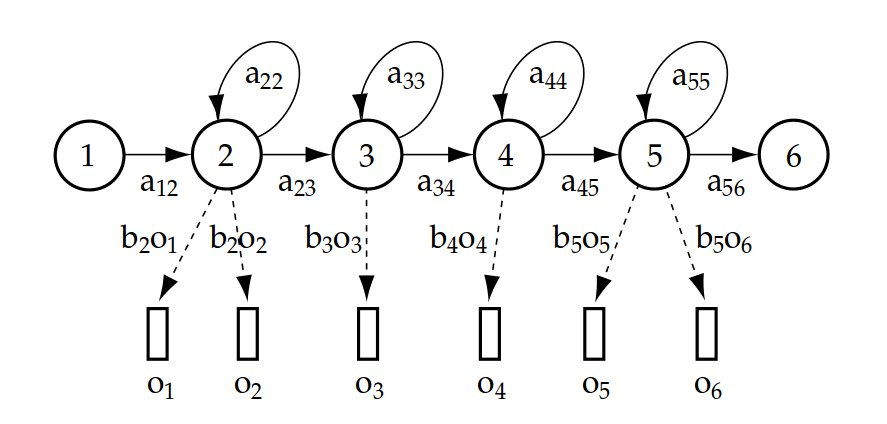
\includegraphics[width=0.7\textwidth]{images/hmm_structure.jpg}
\caption{6-state HMM structure. the states are denoted with numbered circles. State transitions probability form state $i$ to state $j$ are denoted by $a_{ij}$. Output probability densities of state $i$ are denoted $b_{i}$ and the observation generated at time instant $t$ is $o_{t}$}
\label{fig:hmm_structure}
\end{centering}
\end{figure}

Finding the probability that the observed sequence was produced by the given model causes the first problem, but it can be used to score different models based on how well they match the given observation sequence. This probability is calculated by the equation:

\begin{equation}
P(\mathbf{O}|\lambda) = \sum_{all \ Q} P(\mathbf{O}|\mathbf{Q},\lambda) \cdot P(\mathbf{Q}|\lambda)
\end{equation}

Although the calculation of $P(\mathbf{O}|\lambda)$ is straightforward, it involves on the order of $2 \cdot T \cdot N^{T}$ calculations, which is far from being efficient.
%
To reduce the computational cost of this calculation, this problem is usually evaluated with the Forward-Backward algorithm (see \cite{rabiner89}), requiring $N^{2} \cdot T $ calculations.

To solve the second problem we need to find the single best state sequence for a given observation sequence and a given model, i.e. we need to find $Q* = arg max_{Q} P(\mathbf{Q}|\mathbf{O},\lambda)$. 
%
This is usually solved using the Viterbi-algorithm \cite{viterbi67}. 

The third problem listed before is the most difficult one to solve.
%
Solving the model which maximizes the probability of the observation sequence has no known analytical solution. 
%
In stead, gradient based algorithms and iterative algorithms such as the Expectation-Maximization (EM) algorithm \cite{dempster77} are being used for maximizing $P(\mathbf{O}|\lambda)$.

HMMs have the possibility of being extended with various features, increasing the versatility and efficiency depending on the needs of the user. 
%
For example, state tying, state duration densities and inclusion of null transitions are among the extensions proposed.
%
More information about HMMs can be found in  \cite{rabiner89} and \cite{rabiner93}.

\subsection{HMM-Based Speech Synthesis System}
\label{hmm_synthesis_based_system}
In this project an HMM-based speaker-adaptive synthesis system will be used to synthesize speech with different speaker styles.
%
In \cite{tokuda13} a general overview of speech synthesis based in HMMs can be found.

\subsubsection{System Overview}
\label{hmm_synthesis_based_system_overview}
The general overview of a HMM-based synthesis system is ilustrated in Figure \ref{fig:hmm_system_overview}.

\begin{figure}[!htb]
\begin{centering}
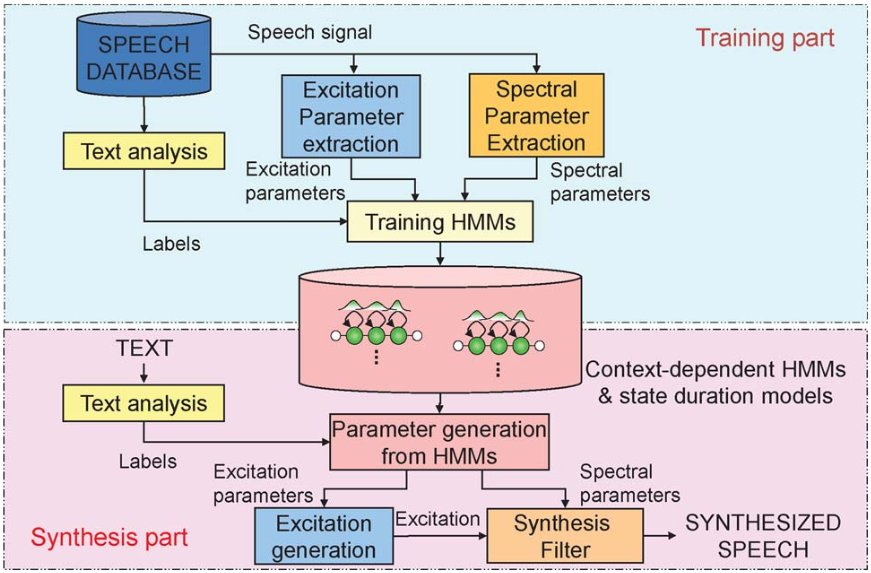
\includegraphics[width=\textwidth]{images/hmm_based_system_overview.jpg}
\caption{Overview of an HMM-based speech synthesis system \cite{tokuda13}}
\label{fig:hmm_system_overview}
\end{centering}
\end{figure}

An HMM-based system can be divided in two major parts: training and synthesis. 